%%%%%%%%%%%%%%%%%%%%%%%%%%%%%%%%%%%%%%%%%
% University/School Laboratory Report
% LaTeX Template
% Version 3.1 (25/3/14)
%
% This template has been downloaded from:
% http://www.LaTeXTemplates.com
%
% Original author:
% Linux and Unix Users Group at Virginia Tech Wiki 
% (https://vtluug.org/wiki/Example_LaTeX_chem_lab_report)
%
% License:
% CC BY-NC-SA 3.0 (http://creativecommons.org/licenses/by-nc-sa/3.0/)
%
%%%%%%%%%%%%%%%%%%%%%%%%%%%%%%%%%%%%%%%%%

%----------------------------------------------------------------------------------------
%	PACKAGES AND DOCUMENT CONFIGURATIONS
%----------------------------------------------------------------------------------------

\documentclass[12pt]{article}

%\usepackage[version=3]{mhchem} % Package for chemical equation typesetting
%\usepackage{siunitx} % Provides the \SI{}{} and \si{} command for typesetting SI units
\usepackage[left=1in,top=1in,right=1in,bottom=1in]{geometry} % Document margins
\usepackage{graphicx} % Required for the inclusion of images
\usepackage{pdfpages}
\usepackage{natbib} % Required to change bibliography style to APA
\usepackage{amsmath} % Required for some math elements 

\setlength\parindent{0pt} % Removes all indentation from paragraphs

\renewcommand{\labelenumi}{\alph{enumi}.} % Make numbering in the enumerate environment by letter rather than number (e.g. section 6)

%\usepackage{times} % Uncomment to use the Times New Roman font

%----------------------------------------------------------------------------------------
%	DOCUMENT INFORMATION
%----------------------------------------------------------------------------------------

\title{\textbf{Find A Room} \\ Design Document \\ CS 307} % Title

\author{Team \textsc{13}(Snoxy)} % Author name

\date{\today} % Date for the report

\begin{document}

\maketitle % Insert the title, author and date

\begin{center}
\begin{tabular}{l r}
Members: & Nathan Chang \\ % Partner names
& Xiaojing Ji \\
& Zilun Mai(Owen) \\
& \textbf{Saranyu Phusit(Team Leader)} \\
& Yao Xiao \\
\\
\bigskip
Instructor: & Professor Buster Dunsmore \\% Instructor/supervisor 
Project Coordinator: & Miguel Villarreal-Vasquez % Instructor/supervisor

\end{tabular}
\end{center}

\newpage
\tableofcontents

% If you wish to include an abstract, uncomment the lines below
% \begin{abstract}
% Abstract text
% \end{abstract}

%----------------------------------------------------------------------------------------
%	SECTION 1
%----------------------------------------------------------------------------------------


\newpage
\section{Purpose}

A mobile application that will give directions indoors by scanning QR codes put on walls throughout a building. The app will direct them towards their destination from where they are.

\subsection{Requirements}
The design should meet the following requirements.

\begin{itemize}
\item Easy to download application. 
\item A QR reader when the application is open.
\item Displaying a map of where they are and locations to map towards.
\item A room search function for rooms that are not on that list.
\item A very fast and easy path finding algorithm.
\item A good display of directions both as a list of directions and a highlighted map.


\end{itemize}



\subsection{General Priority}
The decisions that we make in this document are based on the priorities that we have set for the
project. These are (in order of importance):
\begin{itemize}

\item \textbf{Reliability.} A navigation system MUST be accurate, otherwise the whole entire purpose of it fails. The maps we offer should be accurate enough and have high readability, then the system can locate user’s position and destination accurately which will provide a precise navigation.
\item \textbf{Usability.} Many of our design choices revolved around making it easier for others to use the application. This includes making all maps available and not needing an internet connection, making a very simple interface that makes the goal of each screen clear. We try to let our system be designed in an easy-to-follow pattern, so that users don’t get lost or confused. They can always return to the main menu of this system at any point during navigation.  
\item \textbf{Performance}. Paths and directions need to be calculated as fast as possible to let the user get to their destination as fast as possible. If the path finding is too slow, not much time is saved by using this application than wandering around the floor.
\item \textbf{Portability}. We want to be able to make this application available on all platforms android and iPhone alike. This will allow for all smartphone users to navigate around the campus instead of isolating either android users or iPhone users.
\item \textbf{Reusability}. This program should be able to be used over and over in different buildings while giving the same results. We don’t want this application to be locked into just one building and leave other halls in the dust. 



\end{itemize}
\section{Design Outline}



\subsection{Outline Figures}

To navigate user precisely, we need 3 parts working together: the mobile application, and QR codes covering the area of navigation, and a map.
\\ \\
\textbf{QR code:}
\\
The navigation is based on using QR code to specify the starting point. In each QRcode, the ID of the current node’s ID, and the building ID. Then the app will use the IDs to look up the node inside the building and display corresponding information (e.g. a map for that building it’s on, available destinations, etc.)
\\ \\
\textbf{Mobile Application:}
\\
The mobile application will consist of the QR code reader, the maps of the building and graph representations of each floor. After the QR code is scanned, the app will show available destinations. The path to any destination the user selects can be computed automatically with basic pathfinding algorithm. The app will not require an internet connection. 
\\ \\
\textbf{Map:}
\\
The last necessary components we need is the real map of the floor building. At the initial state, the map and graph representation will be created manually by us. Then if time follows, we will make the process of creating graph representation more automatic for the application to the building outside our scope.


\begin{center}
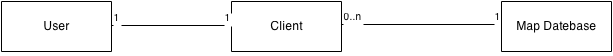
\includegraphics[scale=0.8]{image/user_outline.png}
\end{center}



\section{Design Issue}

We run into several issues.

\subsection{Functional Issue}

\subsubsection{Issue 1}
How to measure the location of the user? \\ \\

Option 1: QR on the wall \\
Option 2: Use bluetooth to measure the distance \\

We choose Option 1 since option 2 needs at least 3 bluetooth devices to determine user’s location and the bluetooth can’t support the distance over 5 meters while the length of a path is usually longer. Option 1 is better since the QR code is easy for user to scan, get information and far cheaper.

\subsubsection{Issue 2}

Where to put QR Code. \\ \\

Option 1: On every destination \\
Option 2: On the corner of the building \\

Although Option 1 will make the path-finding easier, we still decide to use option 2 since the user won’t go through the wrong way when on an edge, and it is a waste of time to put all the QR code on the wall.

\subsubsection{Issue 3}
How should user get the map database? \\ \\

Option 1: Download it with the app. \\
Option 2: Download when user want it. \\

We choose Option 1 since when user needs to use it, he or she must be in hurry of finding a classroom or bathroom so he or she may not have time to download it. 

\subsubsection{Issue 4}
How to let user input their destination? \\ \\
Option 1: We have a list of rooms/ nodes for users to pick while the user inputting their destination. \\
Option 2: We provide a map for user to point at. \\

Option 1 would be our answer. Letting user pointing at the map might be cooler but it’s way more time consuming for user to find their location. Besides the accuracy of pointing would be low. By inputting search bar, it would be quicker and more accurate. 

\subsubsection{Issue 5}
How should the navigation be displayed in the app? \\

Option 1: Display the map of the current building floor and draw out directions with the QR code along as parameters. \\
Option 2: Display current location photo and give direction with text. \\

Option 1 is the way to go.  Our app places accuracy as the most important issue. So we want to make sure our layout is easily understood, and not misleading. If we put it in text and say “Turn right or left within xxx meters”, that would be too vague and misleading. We wanted the user to recognize where they are right now, and how long they need to get to the destination.



\subsection{Non-functional Issue}
\subsubsection{Issue 6}
How should an app be implemented?  \\ \\
Option 1: Native  \\
Option 2: HTML + Phonegap \\

We choose option 2 since our app is not that resource-heavy, implementing it non-natively wouldn’t significantly slow the performance. Also, Option 2 will reduce the development time and allow the app to be made easily cross-platform.



\section{Design Details}
In order to achieve successful indoor navigation, the design of this project will consider a database storing locations of lecture rooms, restrooms, and water fountains. It will also locate the user and navigate them through the inside of the building.  
We decide to apply QR codes and link each QR code to a specific location on the map. Maps has real map images and a list of nodes and edges which represents the map abstractly.  To generate graph of the map, every single node indicates a room, and every edge(with direction) means the length between two nodes. \\ \\
The information will be displayed with half of the screen being a map and the other half being destinations or directions. The top half will include a real image of the map, the path from your location to the destination, and a marker for where you are at the start. The bottom will include a list of notable locations such as bathrooms, water fountains, elevators, and a search function where you can input a room number. \\ \\
The navigation system will calculate the shortest distance between two nodes using graph algorithm. It will calculate the shortest path between two nodes. After it calculates the set of edges the user needs to take, it will return them along with which direction to turn. It will then be presented to the user as a list of instructions on how to get to their destination from where they are. It will also consider other floors and distance that it would take between the floors in the case when there is no bathroom on the current floor as an example.


\subsection{Components}
\textbf{QRcode:}	Each QR code stores its own ID. It will use QR code ID to find the corresponding map, so that users can locate themselves and obtain the floor map by simply scanning and sending the QR code to our app \\ \\
\textbf{Map: }
	Each map can be identified by its own ID named MapID. Since the real map is translated to graph, rooms and water fountains, stairs, elevators, etc. are represented by nodes, the paths between two neighborhoods are represented by edges. NodeList stores every node displayed on the map, as well as EdgeList stores every edge with direction.  MapImg holds the real life map for better user visualization.  The MapImg will be pumped out on the screen once the app successfully identify user’s location and load the corresponding map. 
 For ComputeMap(), once the system gets user’s location and destination on the map, this method helps calculate the total distance by summing up the edges (the paths in real life) among nodes (rooms and public facilities in real) that user will pass. It will find the shortest path using the shortest path algorithm and then return the edges and nodes that a part of this path. The summation can be done by adding the distance values in each edge in the path. \\ \\

\textbf{Path:}	Since every time user can only pick up one destination, eventually the system will provide only one path from current location to destination, this class is a list of edges that will keep all the edges in the right order.  \\ \\

\textbf{Node:}
Each node can be distinguished by its own NodeID, isRoom boolean variable to recognize whether the node is a lecture room or public facilities such as restrooms and water fountains. PosX and PosY record the location of that node, in order to help locate each node on the map to find the optimized path. It also has the floor value.\\ \\
  
\textbf{Edge:}
Edges all have their own ID called EdgeID, and their starting and ending QR code nodes. This object helps ComputePath() to find the path. It will have the distance between the two nodes stored into it. This can be gotten by calculating the distance between the two nodes using their PosX and PosY values. The preview image variable can be used to show an image of their destination instead of an top down map view. The edge will always be a straight line between 2 QR codes.\\ \\

\textbf{Destination:}
Destination is parsed from user’s selection on the lecture rooms list, or public facilities. Each of them can be identified by it DestinationID.\\ \\


\begin{center}
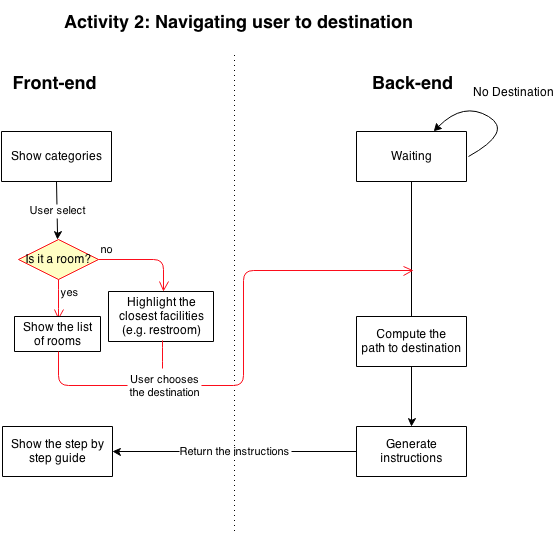
\includegraphics[scale=0.6]{image/image02.png}
\\
\textit{Figure 1. The Class diagram}
\end{center}
\subsection{Process}
We have two main processes for this project. The user should scan the QR code and get the location of the current position, as well as providing the destination( this can be done by selecting one destination from the list we provide or picking public facilities choice)  . The client should provide directions and show the map of current area. The client maps each QR code to a corresponding location of a specific map, thus once it gets the destination, it will set up the connection between the starting point and end point on the map. 

\begin{center}
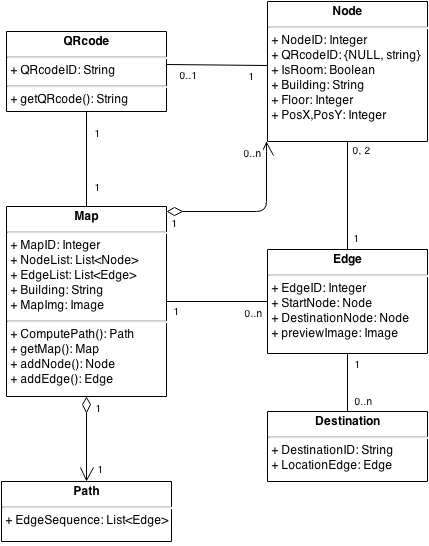
\includegraphics[scale=0.6]{image/image01.png}
\end{center}

Locating where is the User
This allows the application to find where the user is. The application uses a QR code to locate the user once the user scans the QR code.

\begin{center}
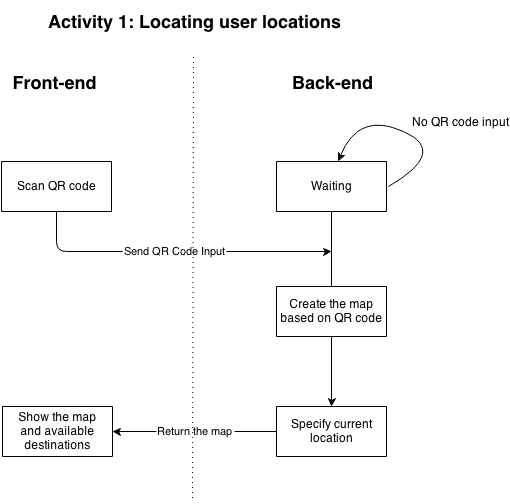
\includegraphics[scale=0.6]{image/image00.png}
\end{center}




\subsection{UI mockup}
Here is the UI mockup showing the 5 main states of an app.

\begin{center}
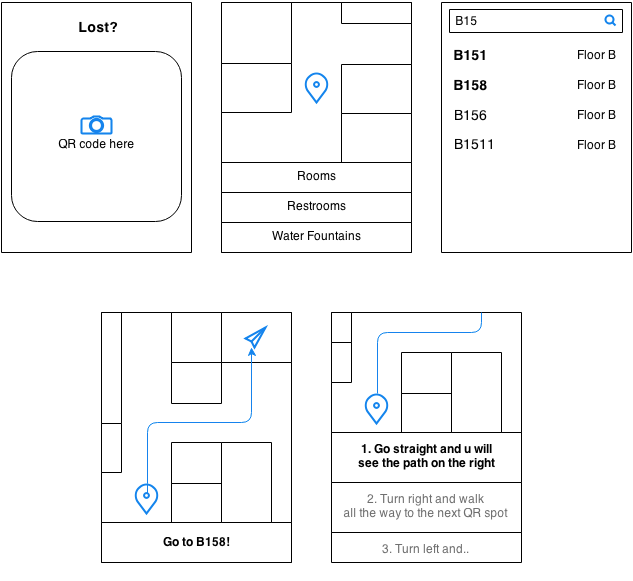
\includegraphics[scale=0.6]{image/image03.png}
\end{center}

\end{document}